\documentclass[11pt]{article}
\usepackage[margin=1in]{geometry}
\usepackage[T1]{fontenc}
\usepackage{lmodern}
\usepackage{microtype}
\usepackage{amsmath,amssymb,amsthm}
\usepackage{booktabs,tabularx,array}
\usepackage{enumitem}
\usepackage{xcolor}
\usepackage{listings}
\usepackage{tikz}
\usetikzlibrary{arrows.meta,positioning}
\usepackage[obeyspaces,spaces]{url}
\usepackage[hidelinks]{hyperref}

\setlist{itemsep=2pt,topsep=4pt}
\setlength{\parskip}{5pt}
\setlength{\parindent}{0pt}
\setlength{\emergencystretch}{3em}
\renewcommand{\arraystretch}{1.25}
\newcolumntype{Y}{>{\raggedright\arraybackslash}X}
\newcolumntype{L}[1]{>{\raggedright\arraybackslash}p{#1}}

\definecolor{codebg}{RGB}{247,247,250}
\definecolor{codeframe}{RGB}{200,200,210}
\definecolor{keyword}{RGB}{30,60,140}
\definecolor{comment}{RGB}{100,110,120}
\definecolor{string}{RGB}{150,60,20}
\definecolor{notebg}{RGB}{238,244,252}
\definecolor{okbg}{RGB}{232,246,234}
\definecolor{warnbg}{RGB}{253,240,232}
\definecolor{linkc}{RGB}{20,80,170}
\definecolor{nodeD}{RGB}{252,232,214}
\definecolor{nodeC}{RGB}{225,238,252}
\definecolor{nodeL}{RGB}{232,246,234}
\hypersetup{colorlinks=true,linkcolor=linkc,urlcolor=linkc,filecolor=linkc}

\lstdefinestyle{java}{language=Java, basicstyle=\ttfamily\small, columns=fullflexible, keepspaces=true,
  keywordstyle=\color{keyword}\bfseries, commentstyle=\color{comment}\itshape, stringstyle=\color{string},
  backgroundcolor=\color{codebg}, frame=single, rulecolor=\color{codeframe}, breaklines=true,
  showstringspaces=false, xleftmargin=4pt, xrightmargin=4pt, aboveskip=6pt, belowskip=6pt}
\lstset{style=java}

\newcommand{\code}[1]{\texttt{#1}}
\newcommand{\shadedbox}[3]{\par\smallskip\noindent\colorbox{#1}{\parbox{\dimexpr\linewidth-2\fboxsep}{\textbf{#2}\par #3}}\par\smallskip}
\newcommand{\takeaway}[1]{\shadedbox{okbg}{In short}{#1}}
\newcommand{\note}[1]{\shadedbox{notebg}{Note}{#1}}
\newcommand{\decision}[1]{\shadedbox{warnbg}{Decision needed}{#1}}
\newcommand{\docsdir}{../}
\def\thisdoc{control}
% Shared cross-document links for the ParaDEVS documents. Each document defines \docsdir (path from its folder to
% docs/) and \thisdoc (its key below), then \input's this file.
%
% \doclink{path relative to docs/}{text}: a link to another PDF. Links are plain URI actions (file:///...), because
% Edge, Chrome and VS Code's PDF viewers ignore hyperref's usual "open another PDF" (GoToR) links. The absolute
% address comes from docroot.tex, which scripts/build_docs.sh regenerates; rerun it if the folder moves.
%
% \relateddocs: the "ParaDEVS documents" box listing every document, with the current one marked.
\InputIfFileExists{\docsdir docroot.tex}{}{\gdef\docroot{.}}
\providecommand{\thisdoc}{}
\definecolor{pdlink}{RGB}{20,80,170}
\definecolor{pdrelbg}{RGB}{243,246,252}
\definecolor{pdrelframe}{RGB}{190,200,220}
\makeatletter
\newcommand{\doclink}[2]{\hyper@linkurl{\textcolor{pdlink}{\textbf{#2}}}{\docroot/#1}}
\newcommand{\pd@item}[4]{% key, path, title, description
  \def\pd@key{#1}%
  \item \ifx\pd@key\thisdoc\textbf{#3} (this document)\else\doclink{#2}{#3}\fi: #4}
\newcommand{\relateddocs}{\par\medskip\noindent
  \fcolorbox{pdrelframe}{pdrelbg}{\parbox{\dimexpr\linewidth-2\fboxsep-2\fboxrule}{\small
  \textbf{ParaDEVS documents.} The entry point is \doclink{ParaDEVS_Start_Here.pdf}{Start Here}, a reading guide
  that links every document.
  \begin{itemize}[leftmargin=1.4em,itemsep=0pt,topsep=2pt]
  \pd@item{report}{report/ParaDEVS_Build_Report.pdf}{Build Report}{what has been built, how it was verified, what is next}
  \pd@item{howto}{howto/ParaDEVS_HowTo.pdf}{How-To Guide}{setup, tutorials, API reference, troubleshooting}
  \pd@item{architecture}{architecture/ParaDEVS_Architecture.pdf}{Architecture Guide}{how the library works and how to read results}
  \pd@item{rl}{rl/ParaDEVS_RL_Plan.pdf}{RL Plan}{reinforcement-learning plan, analysis and results}
  \pd@item{control}{rl/ParaDEVS_Control_Spec.pdf}{Control Spec}{action selection: Para.decide, graph-mode planning, value and policy iteration}
  \pd@item{hybrid}{rl/ParaDEVS_Hybrid_Study.pdf}{Hybrid Study}{which draws to enumerate or sample, and how cost grows with lookahead}
  \pd@item{fastcopy}{engine/ParaDEVS_FastCopy_Proposal.pdf}{Fast-Copy Proposal}{why the engine replays steps, where time goes, how to speed it up}
  \end{itemize}}}\par\medskip}
\makeatother


\theoremstyle{plain}
\newtheorem{proposition}{Proposition}

\title{\textbf{ParaDEVS Control}\\[4pt]\large Specification: the paratemporal engine as a planner for RL action selection,
value iteration and policy iteration (phases 4a--4c)}
\author{ParaDEVS Library workspace, Binghamton}
\date{October 16, 2026}

\begin{document}
\maketitle

\begin{center}
\begin{minipage}{0.88\linewidth}\small
\textbf{How to read this document.} Section~\ref{sec:summary} is a one-page summary. Every later section opens with a
green ``In short'' box, so you can skim by reading only those boxes. Terms are defined in the glossary
(Appendix~\ref{app:glossary}). Background is in the \doclink{rl/ParaDEVS_RL_Plan.pdf}{RL Plan} and the
\doclink{report/ParaDEVS_Build_Report.pdf}{Build Report}.
\end{minipage}
\end{center}

\relateddocs

\tableofcontents
\newpage

%=====================================================================
\section{Summary}\label{sec:summary}

\begin{tabularx}{\linewidth}{@{}>{\bfseries\raggedright\arraybackslash}p{3.3cm}Y@{}}
\toprule
Goal & Use the paratemporal engine to choose actions: at a real state, look $n$ decisions ahead, compute the value
  $e(a)$ of each available action, and act greedily or $\varepsilon$-greedily. The same machinery runs value iteration
  and policy iteration.\\
What a model does & Calls \code{Para.decide(label, obs, options)} for each agent decision (a ``do nothing'' option is
  allowed) and \code{Para.choose} for environment noise, as before. The model does not change between planning,
  policy evaluation and plain MS4 simulation.\\
Key idea & \textbf{Graph mode.} The forward engine sums weights, which suits expectations but cannot take a max.
  The planner instead expands a graph to depth $n$ (merging equal states at equal decision depth), records edges
  with probability, reward and elapsed time, and then runs a backward pass: weighted average at chance nodes, max
  (control) or policy average (evaluation) at decision nodes, leaf values from a batched hook.\\
Time & One step is one decision. DEVS events without a decision are not steps. Discounting is by simulation time,
  $\gamma^{\tau}$ (a semi-MDP); with one time unit per decision this is the usual $\gamma^k$.\\
Guarantees & Exact with exhaustive chance nodes, for the max and for the policy average. With sampled chance nodes
  the policy-weighted value stays unbiased; the sampled max is biased upward (measured; mitigations given).\\
Verified & \textbf{48 new checks pass} (all 147 library checks pass). Depth-$n$ planning equals $n$ steps of value
  iteration at all 64 FrozenLake states to $10^{-16}$; engine-driven policy iteration and value iteration reach $V^*$
  to $3\times10^{-12}$; the merged graph needs $99\times$ fewer simulation runs than the tree at depth 4.\\
Demo & A FrozenLake agent acting by 1-step lookahead with exact $V^*$ leaves reaches the goal in 84--88\% of
  episodes (exact 86.3\%, the optimal policy's rate); with $V=0$ leaves it reaches 0.2\% at depth 1, 7.6\% at depth 8,
  57\% at depth 14.\\
Next & 4d learning comparisons (Python, tabular), 4e the Python wrapper, 4f a DEVS-native problem with random
  event times (Section~\ref{sec:phases}).\\
\bottomrule
\end{tabularx}

\decision{Six questions are listed in Section~\ref{sec:questions}. The most important: (1) whether the safe default
time key (absolute times, merges less) is right, with the relative key as a declared opt-in; (2) the reward-timing
convention for DEVS-native problems; (3) whether the meeting note's $k$-branch estimate $e(a)$ should average over the
policy inside the lookahead (unbiased) or maximize (biased upward).}

\newpage
%=====================================================================
\section{Definitions}\label{sec:defs}

\takeaway{A \emph{decision} is one call to \code{Para.decide}; it is one RL step. Lookahead depth counts decisions,
not DEVS events. Rewards are read from the model's outputs and discounted by elapsed simulation time. What
\code{decide} does depends on who runs the model: it samples a policy in plain MS4, becomes a policy draw in the
forward engine, and becomes a decision node in the planner.}

\paragraph{Decision epoch and step.} A \emph{decision epoch} is the moment a model calls
\code{Para.decide(label, obs, options)} inside a transition. \code{obs} is what the agent observes (the input of the
policy and of the leaf-value hook); \code{options} is the list of available actions, possibly including
\code{Para.NOOP}. Each call is one step, even when only one option exists and even when the option is
\code{NOOP}. DEVS events between two decisions (for example, an environment event or a report) are not steps: they
are part of the transition from one epoch to the next.

\paragraph{Discounting.} A reward output at simulation time $t$ counts $\gamma^{t-t_0}$ from an epoch at time $t_0$.
The next epoch, reached after $\tau$ time units, is discounted by $\gamma^{\tau}$. This is the semi-MDP convention
(discrete lump rewards, continuous time). With $\tau=1$ per decision it is the textbook MDP.

\paragraph{Lookahead to depth $n$.} From a root state, the planner follows every option of every decision and every
outcome (or a sample) of every draw, until $n$ decisions have been made. The state at the next decision epoch is a
\emph{leaf}; its value comes from the \emph{leaf-value hook} $V(\textit{obs})$. A branch that ends (the model becomes
passive) before that is \emph{terminal} and has value 0.

\paragraph{\code{Para.decide} by mode.}
\begin{center}
\small
\begin{tabularx}{\linewidth}{@{}L{3.2cm} Y L{4.4cm}@{}}
\toprule
\textbf{Who runs the model} & \textbf{What \code{decide} does} & \textbf{Used for}\\
\midrule
Plain MS4 simulation & samples an action from the installed policy \code{Para.setPolicy(p)}; the default is uniform
  over the options & running an agent; acting (a lookahead policy can be installed)\\
Forward engine (\code{ParaEngine}) & a draw from the installed policy's law; exhaustive, sampled or hybrid like any draw
  & policy evaluation with the full return distribution; n-step targets\\
Planner, \emph{evaluate} & decision node; backward pass takes $\sum_a \pi(a\mid \textit{obs})\,Q(a)$ & $Q^\pi$, $V^\pi$;
  policy iteration's evaluation step\\
Planner, \emph{control} & decision node; backward pass takes $\max_a Q(a)$ & value iteration; expectimax lookahead\\
\emph{Act} (online) & plan from the real state with control (or evaluate), report $e(a)=Q(a)$ for every option, pick
  greedily or $\varepsilon$-greedily & online action selection\\
\bottomrule
\end{tabularx}
\end{center}
At the root decision the planner always reports $Q(a)$ for every option, whichever rule is used below it.

\paragraph{Targets.} With $V$ the learner's values at the leaves:
\begin{center}
\small
\begin{tabularx}{\linewidth}{@{}L{3.6cm} Y L{4.4cm}@{}}
\toprule
\textbf{Target} & \textbf{Backward pass} & \textbf{Standard counterpart}\\
\midrule
Policy-weighted & policy average at every decision, leaf $V(s)$ & $n$-step Expected SARSA, tree backup, $V^\pi$
  evaluation\\
Max at the leaves & policy average inside, leaf $\max_a Q(s,a)$ (a hook choice) & $n$-step Q-learning-style targets\\
Max inside the tree & max at every decision & $n$ steps of value iteration, expectimax\\
\bottomrule
\end{tabularx}
\end{center}

%=====================================================================
\section{Graph mode}\label{sec:graph}

\takeaway{The planner turns the simulation into a layered graph. Nodes that reach the same model state at the same
decision depth are merged, because their future value is the same. Rewards and elapsed times sit on the edges, not in
the nodes. One backward sweep then computes every value. The expensive part, simulation, is done once; the cheap
backward pass can be repeated with new leaf values.}

\begin{center}
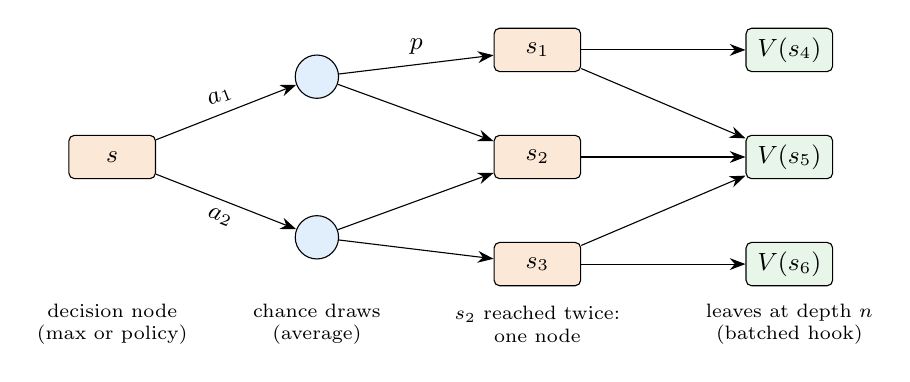
\begin{tikzpicture}[x=1.0cm,y=0.85cm,font=\small,
  dn/.style={draw,rounded corners=2pt,fill=nodeD,minimum width=1.1cm,minimum height=0.55cm},
  cn/.style={draw,circle,fill=nodeC,minimum size=0.55cm,inner sep=0pt},
  ln/.style={draw,rounded corners=2pt,fill=nodeL,minimum width=1.1cm,minimum height=0.55cm},
  e/.style={-{Stealth[length=2mm]}}]
\node[dn] (r) at (0,0) {$s$};
\node[cn] (a) at (2.6,1.2) {};
\node[cn] (b) at (2.6,-1.2) {};
\node[dn] (x) at (5.4,1.6) {$s_1$};
\node[dn] (y) at (5.4,0) {$s_2$};
\node[dn] (z) at (5.4,-1.6) {$s_3$};
\node[ln] (l1) at (8.6,1.6) {$V(s_4)$};
\node[ln] (l2) at (8.6,0) {$V(s_5)$};
\node[ln] (l3) at (8.6,-1.6) {$V(s_6)$};
\draw[e] (r) -- node[above,sloped] {$a_1$} (a);
\draw[e] (r) -- node[below,sloped] {$a_2$} (b);
\draw[e] (a) -- node[above] {$p$} (x);
\draw[e] (a) -- (y);
\draw[e] (b) -- (y);
\draw[e] (b) -- (z);
\draw[e] (x) -- (l1); \draw[e] (x) -- (l2);
\draw[e] (y) -- (l2); \draw[e] (z) -- (l2); \draw[e] (z) -- (l3);
\node[font=\scriptsize,align=center] at (0,-2.5) {decision node\\(max or policy)};
\node[font=\scriptsize,align=center] at (2.6,-2.5) {chance draws\\(average)};
\node[font=\scriptsize,align=center] at (5.4,-2.5) {$s_2$ reached twice:\\one node};
\node[font=\scriptsize,align=center] at (8.6,-2.5) {leaves at depth $n$\\(batched hook)};
\end{tikzpicture}
\end{center}

\paragraph{Nodes.}
\begin{itemize}
\item \textbf{Chance node}: a persistent model state (a completed departure) at decision depth $d$, after $e$ events
  since the last decision. Its next event may make draws; each outcome (or sample) leads to another chance node or to
  a decision node.
\item \textbf{Decision node}: a departure suspended at \code{decide}. Each option is resumed; the rest of the
  departure may make more draws. It is a leaf when $d=n$.
\item \textbf{Edge}: (child, weight $w$, reward $r$, elapsed time $\Delta t$). The weight is the probability (exhaustive)
  or the sample factor $1/k$ (sampled); $r$ is the discounted reward of the departure.
\end{itemize}

\paragraph{Merge keys.} The key holds no accumulated reward: rewards are on the edges, so a node's value depends only
on its state and on the remaining depth $n-d$. Under the Markov property and additive rewards this is exact for both
the expectation and the max.
\begin{itemize}
\item Chance node: (model state key, $d$, $e$). Including $e$ makes the graph layered and acyclic.
\item Decision node: (pre-departure state key, event kind, values already drawn in this departure, $d$). It does not
  include $e$, so paths with different numbers of intermediate events still meet at their next decision.
\end{itemize}

\paragraph{Time in the key.} The library's state key includes the simulator's last and next event times, which are
absolute. Two settings (\code{PlanSpec.TimeKey}):
\begin{itemize}
\item \textbf{ABSOLUTE} (default): the node time and absolute event times are in the key. Sound for every model, but
  states reached at different times never merge.
\item \textbf{RELATIVE} (declared opt-in): times are taken relative to the node time: the time to the next event
  $t_N-t$ for each component, and the elapsed time $t-t_L$ for components of a coupled model (they can receive inputs,
  and an external transition sees the elapsed time). A top-level atomic model receives no inputs under the planner,
  so its elapsed time cannot matter and is left out. This is sound for \emph{time-homogeneous} models: transitions do
  not read the absolute clock except through model fields, and fields are always in the key (a field holding an
  absolute time just prevents merges). With random event times it matters: in the semi-MDP check the relative key
  needs 1{,}265 nodes and the absolute key 7{,}584 (Section~\ref{sec:verify}).
\end{itemize}
A model that supplies its own key (\code{ParaStateKey}) can leave out \code{sigma}: its only role is the time advance,
which the key already holds as the next event time.

\paragraph{Processing order.} Nodes are expanded in the order (depth $d$; chance nodes before decision nodes; $e$).
Every edge leads to a later node, so each node is expanded once, after all its arrivals, and a budget rule sees its
full reach weight.

\paragraph{Backward pass.} In reverse order,
\begin{align*}
\text{chance node:}\quad & V(u)=\sum_{\text{edges }u\to c} w\,\big(r+\gamma^{\Delta t}V(c)\big),\\
\text{decision node:}\quad & Q(u,a)=\sum_{\text{edges of }a} w\,\big(r+\gamma^{\Delta t}V(c)\big),\qquad
  V(u)=\textsc{rule}\big(Q(u,\cdot)\big),
\end{align*}
with leaves $V(u)=\textit{hook}(\textit{obs}_u)$ and terminals $V(u)=0$. The hook is called \textbf{once per backward
pass} with every distinct leaf observation, so a Python learner is called once per plan.

%=====================================================================
\section{Guarantees}\label{sec:guarantees}

\takeaway{With every outcome enumerated, the planner's values are exactly those of dynamic programming. With sampled
outcomes, the policy-weighted value is still correct on average. The sampled max is not: it is too optimistic on
average, because the max picks up lucky samples. The fixes are to enumerate small draws, to sample more, or to choose
and evaluate with independent samples.}

Conditions throughout: finite option lists, finitely many draws per departure, finite-support laws for enumerated
draws, a deterministic departure given the state and the supplied values (the library's standing requirement), and
rewards that add along a path.

\begin{proposition}[Exact with exhaustive chance nodes]
With exhaustive selection, the backward pass with the max rule and $V=V_0$ at the leaves gives
$V(\text{root})=(T^n V_0)(s)$, where $T$ is the Bellman optimality operator of the (semi-)MDP the model defines. With
the policy rule it gives $(T_\pi^n V_0)(s)$. Root $Q(a)$ values are those of $T^{n-1}V_0$ (or $T_\pi^{n-1}V_0$).
\end{proposition}
\emph{Why.} Without merging, the graph is the expectimax tree, whose backward pass is $T$ applied $n$ times, by
induction on the remaining depth. A merged node stands for several tree nodes whose futures are equal: equal keys
mean equal continuation laws (safe merging, main\_paratemporal Prop.~``Safe merging''), the same remaining depth, and
no dependence on the path's past reward, since rewards are on the edges. Their tree values are therefore equal, and
the merged node's single value can be used for all. The edges keep their own $w$, $r$ and $\Delta t$, so nothing
path-dependent is lost. The max is applied to values that are each exact, so it is exact as well.

\begin{proposition}[Unbiased policy-weighted target with sampled chance nodes]
With any selection rule whose sample factors satisfy $E[\sum_i \alpha_i f(v_i)] = E_P f$ (exhaustive,
\code{monteCarlo(k)}, \code{budget(B)}, hybrid by label), and with the policy rule, $E[\hat V(\text{root})]
=(T_\pi^n V_0)(s)$, also with merging.
\end{proposition}
\emph{Why.} The backward pass is linear in the leaf values and in the edge weights when the rule is the policy
average. Conditionally on everything before a node is expanded, its draws are fresh, so the expected value of its
estimate is its true value, by induction from the leaves. Merging only shares an expansion between parents; each
parent's expectation is unchanged. This is the forward engine's argument (main\_paratemporal, sampled case), applied
backward.

\begin{proposition}[Upward bias of the sampled max]
With sampled chance nodes and the max rule, $E[\hat V] \ge V$, with strict inequality when the action ranking can
change between samples.
\end{proposition}
\emph{Why.} Each $\hat Q(a)$ is unbiased, and $E[\max_a \hat Q(a)] \ge \max_a E[\hat Q(a)]$ (Jensen; the max is
convex). Inside the tree the bias compounds, because each max sees already-optimistic children. This is the
optimizer's curse, the same effect behind maximization bias in Q-learning.

\paragraph{Measured} (FrozenLake, state 18, $V^*$ leaves, so the exact value is $V^*(18)=0.3755$; 200 seeds).
\begin{center}
\small
\begin{tabular}{@{}lrrr@{}}
\toprule
\textbf{Chance nodes} & \textbf{Mean} & \textbf{Bias} & \textbf{s.e.}\\
\midrule
exhaustive, depth 3 & 0.375496 & 0 (exact) & 0\\
\code{monteCarlo(1)}, depth 1 & 0.4119 & $+0.036$ & 0.0026\\
\code{monteCarlo(3)}, depth 1 & 0.3919 & $+0.016$ & 0.0020\\
\code{monteCarlo(3)}, depth 3 & 0.4103 & $+0.035$ & 0.0017\\
double estimation at the root, $k=1$, depth 1 & 0.3169 & $-0.059$ & 0.0106\\
\bottomrule
\end{tabular}
\end{center}
\paragraph{Mitigations.}
\begin{enumerate}
\item \textbf{Enumerate small draws} (hybrid selection: \code{exhaustive} on labels with few outcomes, sampling on
  the rest). Where every draw is enumerated, the bias is zero. This is the engine's main advantage over plain
  sampling-based planners (Build Report and RL Plan: exhaustive expansion with merging wherever outcome sets are small).
\item \textbf{Sample more}: the bias shrinks as $k$ or $B$ grows ($+0.036\to+0.016$ from $k=1$ to $k=3$ at depth 1).
\item \textbf{Double estimation}: select the action with one sampled plan and evaluate it with an independent one
  (double Q-learning). It removes the upward bias (it may err downward, as measured). At the root this is two plans;
  inside the tree it needs two independent sample sets per node (future work).
\item \textbf{Use the policy rule for targets}: for learning targets, the policy-weighted target is unbiased; keep the
  max for action selection, where only the ranking matters.
\end{enumerate}

%=====================================================================
\section{API}\label{sec:api}

\takeaway{A model calls \code{Para.decide}. A caller builds a \code{PlanSpec}, expands a \code{Plan} from one or many
roots, and runs \code{backup} with a rule and leaf values. All inputs and outputs are lists and arrays, so the Python
side can call it in batches. A \code{LookaheadPolicy} lets an agent act by planning inside a plain MS4 run.}

\paragraph{Model side} (\path{examples/rl/MdpAgent.java}, abridged).
\begin{lstlisting}
if (phase == Phase.DECIDE) {
    Object a = Para.decide("action", s, options());     // one RL step
    int s2 = a == Para.NOOP ? s
           : Para.choose("transition", mdp.transitionLaw(s, (Integer) a));
    reward = a == Para.NOOP ? 0 : mdp.rewardOnArrival(s2);
    s = s2; phase = Phase.REPORT; sigma = 0;           // report at the same time
} else if (phase == Phase.REPORT) {                    // an event, not a step
    reward = 0;
    if (mdp.isTerminal(s)) { phase = Phase.DONE; sigma = INFINITY; }
    else { phase = Phase.DECIDE; sigma = duration(); } // 1, or a "duration" draw
}
\end{lstlisting}

\paragraph{Planning side} (package \code{paradevs.engine}).
\begin{lstlisting}
PlanSpec spec = PlanSpec.depth(n)              // n decisions ahead
    .gamma(0.99)                               // per unit of simulation time
    .selection(SelectionRule.exhaustive())     // or monteCarlo(k), budget(B), hybrid
    .timeKey(PlanSpec.TimeKey.RELATIVE);       // opt-in: time-homogeneous models

Plan plan = Planner.expandFresh(spec, roots);  // many roots, one shared graph
List<Object> obs = plan.leafObservations();    // distinct leaf observations
Plan.Values v = plan.backup(DecisionRule.max(), leafValues);  // double[], as obs
// or: plan.backup(DecisionRule.policy(pi), LeafValues.table(V))

double value = v.value(i);                     // V(root i)
double[] q   = v.q(i);                         // e(a) = Q(root decision, a)
List<?> acts = v.actions(i);                   // the options, in model order
double[] p   = v.epsilonGreedy(i, 0.1, 1e-12); // epsilon-greedy, ties shared
Plan.Stats w = plan.stats();                   // departures, nodes, merged, ms
\end{lstlisting}
Other pieces: \code{Planner.Root.snapshot(model, now)} plans from a model in the middle of a plain MS4 run;
\code{PlanSpec.prune(pi)} expands only the actions a policy can take (below the root); \code{PlanSpec.merge(false)}
gives the plain tree, for comparison. \code{Para.Policy} is
\code{double[] probabilities(label, obs, options)}; \code{LeafValues} is \code{double[] values(List<Object> obs)} (a
batch), with \code{LeafValues.of(v)} for a single-leaf function, \code{table(v)} and \code{zero()}.

\paragraph{Acting under plain MS4.} Install a lookahead policy; every \code{decide} then plans from the current
observation.
\begin{lstlisting}
Planner.LookaheadPolicy act = Planner.lookahead(
    PlanSpec.depth(1).gamma(0.99),
    obs -> new MdpAgent("frozenLake8x8", (Integer) obs),  // first decision at obs
    DecisionRule.max(), LeafValues.table(vStar),
    0.0,                                                  // epsilon
    true);                                                // cache by observation
act.prepare(allStates);      // optional: one batched plan for many states
Para.setPolicy(act);         // then run the model in MS4 as usual
\end{lstlisting}
Without an installed policy, \code{decide} under plain MS4 samples uniformly over the options (documented default).
The cache is valid with exhaustive selection and fixed leaf values, where a plan never changes.

\paragraph{From Python} (sketch; the wrapper is being built separately, phase 4e).
\begin{lstlisting}[language=Python]
plan = Planner.expandFresh(spec, roots)        # roots built on the Java side
obs  = list(plan.leafObservations())
leaf = JArray(JDouble)(learner.V(obs))         # one learner call per plan
vals = plan.backup(DecisionRule.max(), leaf)
q    = np.array(vals.q(0))                     # e(a) at the real state
\end{lstlisting}

%=====================================================================
\section{How it plugs into value iteration, policy iteration and acting}\label{sec:plug}

\takeaway{Expand once, back up many times. Value iteration repeats the max backup with the previous values at the
leaves; policy iteration alternates policy backups (evaluation) with a greedy choice from the root $Q$ values
(improvement); acting plans from the real state and picks from $e(a)$.}

\begin{itemize}
\item \textbf{Value iteration.} Expand a depth-$n$ plan from every state (one shared graph). Iterate
  $V_{k+1}(s)=$ \code{backup(max, }$V_k$\code{).value(s)}; each sweep applies $T^n$. No simulation is repeated.
\item \textbf{Policy iteration.} Evaluation: iterate the policy backup to a fixed point (or use the forward engine for
  the whole return distribution). Improvement: $\pi'(s)=\arg\max_a$ \code{q(s)[a]} with the leaves at $V^\pi$, keeping
  the current action on ties.
\item \textbf{Online action selection} (the priority). At the real state, plan to depth $n$ with the learner's $V$ at
  the leaves, read $e(a)=Q(a)$ for every option, and act greedily or $\varepsilon$-greedily. The meeting note's ``play
  each action forward $k$ times'' is \code{selection(monteCarlo(k))} with \code{merge(false)}; merging and enumeration
  of small draws are the engine's additions. Learners remain standard: the engine supplies $e(a)$, the learner
  updates $V$ or $Q$ from real transitions (or from engine targets).
\item \textbf{$n$-step targets for TD learning.} The policy backup at a real state gives an unbiased $n$-step expected
  target, generalizing the existing forward-engine targets (\code{NStepTargets}) to models with agent decisions.
\end{itemize}

%=====================================================================
\section{Verification (phase 4c)}\label{sec:verify}

\takeaway{The planner was checked against exact dynamic programming on the 19-state random walk and slippery
FrozenLake $8\times8$. Every exact check matches to $10^{-12}$ or better, the merged graph is far cheaper than the
tree, the sampled estimators behave as Section~\ref{sec:guarantees} predicts, and the online demo reaches the optimal
success rate. Test: \code{bash scripts/build\_library.sh control} (about one minute).}

\begin{center}
\small
\begin{tabularx}{\linewidth}{@{}Y L{4.4cm} r@{}}
\toprule
\textbf{Check} & \textbf{Result} & \textbf{Work}\\
\midrule
Depth $n$, $V=0$, max: $V$ and $Q$ = $n$ steps of VI at every state; random walk $n=1,5,12$ & error 0 & 137--1{,}204\\
Same, FrozenLake $\gamma=0.99$, $n=1,3,10$, all 64 states & error $\le 1.1\times10^{-16}$ & 1{,}076--9{,}707\\
Same, with a no-op action ($n=4$), against DP with a ``stay'' action & error $\le 1.1\times10^{-16}$ & \\
Semi-MDP: step durations $\{0.5,1,2\}$ w.p.\ $\{\tfrac14,\tfrac12,\tfrac14\}$, $\gamma=0.9$, $n=4$, both time keys
  & error $2.8\times10^{-17}$ & 5{,}013 (rel.), 33{,}477 (abs.)\\
Uniform $\pi$, depth 2, $V^\pi$ leaves: $V^\pi$, $Q^\pi$, greedy improvement & $1.8\times10^{-13}$, $9.1\times10^{-14}$,
  53/53 states agree & \\
Policy iteration on one depth-1 graph, from ``always Left'' & 11 improvements, 6{,}944 backups;
  $|V-V^*|\le3.0\times10^{-12}$, optimal policy & 1{,}076\\
Value iteration on the same graph & 1{,}027 backups; $|V-V^*|\le3.0\times10^{-12}$ & 1{,}076\\
\code{decide} under the forward engine (policy draws) vs the planner, $n=3$ & equal to $10^{-15}$; both $=V^\pi(18)$ & \\
Plan from a model in the middle of a plain MS4 run (\code{Root.snapshot}) vs a fresh model & $Q$ equal (error 0) & \\
\code{decide} under plain MS4 with the default policy & the episode runs to its end & \\
Sampled, policy rule: \code{monteCarlo(3)}, \code{budget(12)}, hybrid (durations sampled) & unbiased, within
  0.7, 0.9, 1.6 s.e. & 237, 861\\
Sampled, max rule & upward bias measured (Section~\ref{sec:guarantees}) & \\
\bottomrule
\end{tabularx}
\end{center}
Work counts departures (simulation runs of one event, including replays).

\paragraph{Graph versus tree} (FrozenLake, state 18, the same value to $10^{-12}$).
\begin{center}
\small
\begin{tabular}{@{}lrrrr@{}}
\toprule
\textbf{Depth} & \textbf{Graph departures} & \textbf{Graph nodes} & \textbf{Tree departures} & \textbf{Ratio}\\
\midrule
2 & 89 & 37 & 399 & $4.5\times$\\
4 & 478 & 143 & 47{,}379 & $99\times$\\
\bottomrule
\end{tabular}
\end{center}
The tree grows like $12^n$ (4 actions, 3 slips); the graph grows linearly in $n$, bounded by the number of states per
depth. A depth-10 plan from all 64 states takes 9{,}707 departures, about one second.

\paragraph{Online action selection demo} (FrozenLake $8\times8$, plain MS4 simulation, the agent calls
\code{decide} and a \code{LookaheadPolicy} plans; greedy, ties shared; success = goal within 200 decisions; 500
episodes; the exact rate of each induced policy by DP).
\begin{center}
\small
\begin{tabular}{@{}lrrrr@{}}
\toprule
\textbf{Leaves, depth} & \textbf{Simulated} & \textbf{Exact} & \textbf{$e(a)$ at the start (L, D, R, U)} & \textbf{Plan departures}\\
\midrule
$V^*$, $n=1$ & 0.840 & \textbf{0.8630} & 0.4095, 0.4137, 0.4137, 0.4146 & 1{,}076\\
$V^*$, $n=3$ & 0.884 & \textbf{0.8630} & same & 2{,}994\\
$V=0$, $n=1$ & 0.002 & 0.0024 & 0, 0, 0, 0 & 1{,}076\\
$V=0$, $n=4$ & 0.016 & 0.0132 & 0, 0, 0, 0 & 3{,}953\\
$V=0$, $n=8$ & 0.076 & 0.0932 & 0, 0, 0, 0 & 7{,}789\\
$V=0$, $n=14$ & 0.572 & 0.5709 & 0, 0, 0, 0 & 13{,}543\\
$V=0$, $n=30$ & 0.702 & 0.7191 & 0.0230, 0.0276, 0.0276, 0.0284 & 28{,}887\\
\bottomrule
\end{tabular}
\end{center}
With exact leaves, one step of lookahead already gives the optimal policy (for $\gamma=0.99$), whose success rate is
0.863. With $V=0$ the agent sees nothing until the goal is within $n$ decisions; the goal is 14 steps from the start, so
small $n$ is nearly random. This is the gap a learned $V$ is meant to close (phase 4d). All plans for the 64 states
were computed in one batched call and cached.

%=====================================================================
\section{Phase plan}\label{sec:phases}

\takeaway{4a--4c are done (this document, the engine and the exact checks). Next is the learning comparison in
Python, the Python wrapper, and a problem where DEVS time matters.}

\begin{center}
\small
\begin{tabularx}{\linewidth}{@{}L{2.1cm} Y L{4.0cm}@{}}
\toprule
\textbf{Phase} & \textbf{Work} & \textbf{Done when}\\
\midrule
4a Spec & this document & reviewed by the user and advisor\\
4b Engine & \code{Para.decide}, \code{Planner}, \code{Plan}, \code{PlanSpec}, \code{LeafValues}, \code{DecisionRule},
  \code{LookaheadPolicy}; \code{MdpAgent} model & done; all tests pass\\
4c Exact DP checks & \code{VerifyControl} (48 checks, Section~\ref{sec:verify}) & done\\
4d Learning comparisons & Tabular learners in Python (Q-learning, $n$-step SARSA, Expected SARSA / tree backup) on the
  random walk and FrozenLake, against the same learners helped by the engine: (i) action selection by lookahead with
  the learned $V$ at the leaves; (ii) engine $n$-step targets; (iii) $k$-branch $e(a)$ (sampled) vs exhaustive with
  merging. Measures: return and value error per real episode, and per unit of compute (departures), at equal compute;
  $\varepsilon$-greedy over $e(a)$ & learning curves with confidence bands; a compute-normalized comparison\\
4e Python & JPype wrapper: \code{plan(states, n, rule, leaf\_fn)} returning $e(a)$ arrays; a Gymnasium environment
  whose \code{step(action)} runs the MS4 model; one learner call per plan & Python reproduces the 4c numbers\\
4f DEVS-native problem & T4 of the RL Plan: admission control or an $(s,S)$ inventory with random event times, several
  events between decisions, a coupled model, the relative time key & DP on the embedded chain matches; learning
  comparison repeated\\
\bottomrule
\end{tabularx}
\end{center}
Later: neural networks for $V$ (the batched hook is designed for this); double estimation inside the tree;
expectation-only merging for the forward engine (being added separately) used for policy-weighted targets.

%=====================================================================
\section{Open questions}\label{sec:questions}

\takeaway{Six choices were made to get a working first version. Each is safe, but the user or advisor should confirm
or change them.}

\begin{enumerate}
\item \textbf{Time key default.} ABSOLUTE is sound for every model but merges less; RELATIVE must be declared and is
  sound for time-homogeneous models. Keep this default?
\item \textbf{Reward timing.} \code{MdpAgent} reports the reward at the decision time, so the textbook MDP is recovered
  with $\tau=1$. In a semi-MDP, rewards earned at the end of a sojourn would be discounted by $\gamma^{\tau}$. Which
  convention for DEVS-native problems (lump sums when output, or reward rates)?
\item \textbf{The meeting note's $e(a)$.} Should the $k$-branch estimate average over the policy below the first action
  (unbiased) or maximize (biased upward, Section~\ref{sec:guarantees})? The API supports both.
\item \textbf{Leaf input.} The hook receives the \code{obs} passed to \code{decide}. That is right when \code{obs} is a
  Markov state; for partially observed DEVS models the hook may need the model state instead.
\item \textbf{Default policy under plain MS4.} Uniform over the options. Alternatives: the first option, or an error
  when no policy is installed.
\item \textbf{Merging across event counts.} Chance nodes include the number of events since the last decision, so the
  graph is acyclic; decision nodes do not. Merging chance nodes across event counts would need cycle handling. Is the
  current trade-off acceptable?
\end{enumerate}

\appendix
%=====================================================================
\section{Glossary}\label{app:glossary}
\begin{tabularx}{\linewidth}{@{}>{\bfseries\raggedright\arraybackslash}p{3.6cm}Y@{}}
\toprule
Decision (step) & One call to \code{Para.decide}; one RL step.\\
Decision epoch & The moment of a decision, with its observation and options.\\
No-op & The ``do nothing'' option \code{Para.NOOP}; choosing it is still a step.\\
Draw & One call to \code{Para.choose}: a random value with a known law (environment noise).\\
Departure & One run of one DEVS event from a saved state; the unit of work.\\
Chance node & A model state between decisions; its draws are averaged.\\
Decision node & A suspended \code{decide}; its options are maximized over or averaged by a policy.\\
Leaf & A decision node after $n$ decisions; valued by the leaf-value hook.\\
Terminal & A branch whose model became passive; value 0.\\
Merge key & What two nodes must share to be joined: state, decision depth (and, for chance nodes, events since the
  last decision).\\
Time key & Whether times enter the key as absolute values or relative to the node time.\\
Backward pass (backup) & The sweep from leaves to roots that computes all values.\\
$e(a)$, $Q(s,a)$ & The value of taking action $a$ now and then following the rule.\\
Policy-weighted target & Values averaged over the policy at every decision; unbiased under sampling.\\
Value iteration & Repeating the max backup until values stop changing; gives $V^*$.\\
Policy iteration & Alternating evaluation of a policy and greedy improvement.\\
$\varepsilon$-greedy & Act on the best $e(a)$ with probability $1-\varepsilon$, uniformly otherwise.\\
Semi-MDP & An MDP in which steps take random time; discounting by $\gamma^{\tau}$.\\
Selection rule & How draws are expanded: exhaustive, \code{monteCarlo(k)}, \code{budget(B)}, hybrid by label.\\
Optimizer's curse & The max of noisy estimates is too high on average.\\
Double estimation & Choosing with one estimate and evaluating with an independent one.\\
Expectimax & A lookahead tree with max at decisions and averages at chance nodes.\\
MDP homomorphism & A map to a smaller MDP that preserves transitions and rewards; exact merging is a special case.\\
\bottomrule
\end{tabularx}

\end{document}
